\section{Introduction}
Robots operating in real-world scenarios demand a delicate balance between adaptability and reactivity. While the robot must efficiently accomplish its designated tasks, it is equally essential to ensure the safety of its movements by avoiding collisions at all times. In contemporary robotic applications, there is a growing emphasis on achieving increased physical human-robot collaboration \cite{ajoudani2018progress}.
% Robots moving in real-world scenarios need to be adaptable and reactive. While on the one hand, the robot needs to complete its motion, on the other hand, its movement must be safe, i.e., it can avoid collisions at all times. Modern robotic applications require increased physical human-robot collaboration \cite{ajoudani2018progress}.

Central to controlling a robot is the task of planning a trajectory that guides it towards a desired goal. Trajectories in complex environments often necessitate easily parametrizable methods. Human demonstration stands out as an intuitive approach to instruct robots on desired actions, enabling the sequencing of simple movements to generate intricate motions \cite{gribovskaya2011motion}. 
A closed-form control law that obviates the need for constant replanning at every position is desirable. In this context, Dynamical Systems (DS) control emerges as a promising technique, offering stability and convergence guarantees for navigation in dynamic environments.
%One of the big tasks of controlling a robot is planning a trajectory to reach a desired goal. Trajectories can often be very complex, and one has to find methods to parametrize those easily. The human demonstration is an easy way of showing the robot what to do. Simple movement can be sequenced to generate a complex motion \cite{gribovskaya2011motion}.

% It has a closed-form control law that does not require constant replanning for every position. In addition, DS control can provide stability and convergence guarantees for navigation in dynamic environments. Applications that involve interactions with an unknown and dynamic environment, for example, manipulation around humans, require controllers for actuators that are not which exceed classical stiffness controllers.

However, certain robotic applications, especially when involving interactions with unknown and dynamic environments, such as manipulation around humans, call for novel controllers that surpass traditional stiffness controllers. Biological systems, with their remarkable functional and neuro-mechanical control, outperform conventional mechanical devices. Notably, the adaptability and variable stiffness exhibited by biological muscles contrast with the performance of rigid electrical drives commonly employed in industrial robotics. These stiff drives rely on precise reference-trajectory tracking, whereas biological systems exhibit inherent flexibility and adaptability.
% Biological muscles outperform mechanical devices in terms of functional and neuro-mechanical control. One key distinction is the adaptable compliance or variable stiffness exhibited in biological systems, which contrasts with the performance of traditional stiff electrical drives commonly used in industrial robotics. Unlike these drives, which rely on precise reference-trajectory tracking, biological systems possess inherent flexibility and adaptability.

Incorporating obstacle avoidance into reactive motion controllers remains a crucial challenge. When designed correctly, impedance controllers maintain stable motion and ensure collision avoidance by limiting the force applied to external obstacles below a specified threshold. Nevertheless, to enhance overall behavior, it is essential for the robot to proactively avoid collisions before they occur, even while impedance control operates in fail-safe interaction mode. Furthermore, in specific scenarios, it becomes critical for the robot to effectively reject disturbances (Fig.~\ref{fig:table_avoidance_with_obstacle}). 

\begin{figure}
\centerline{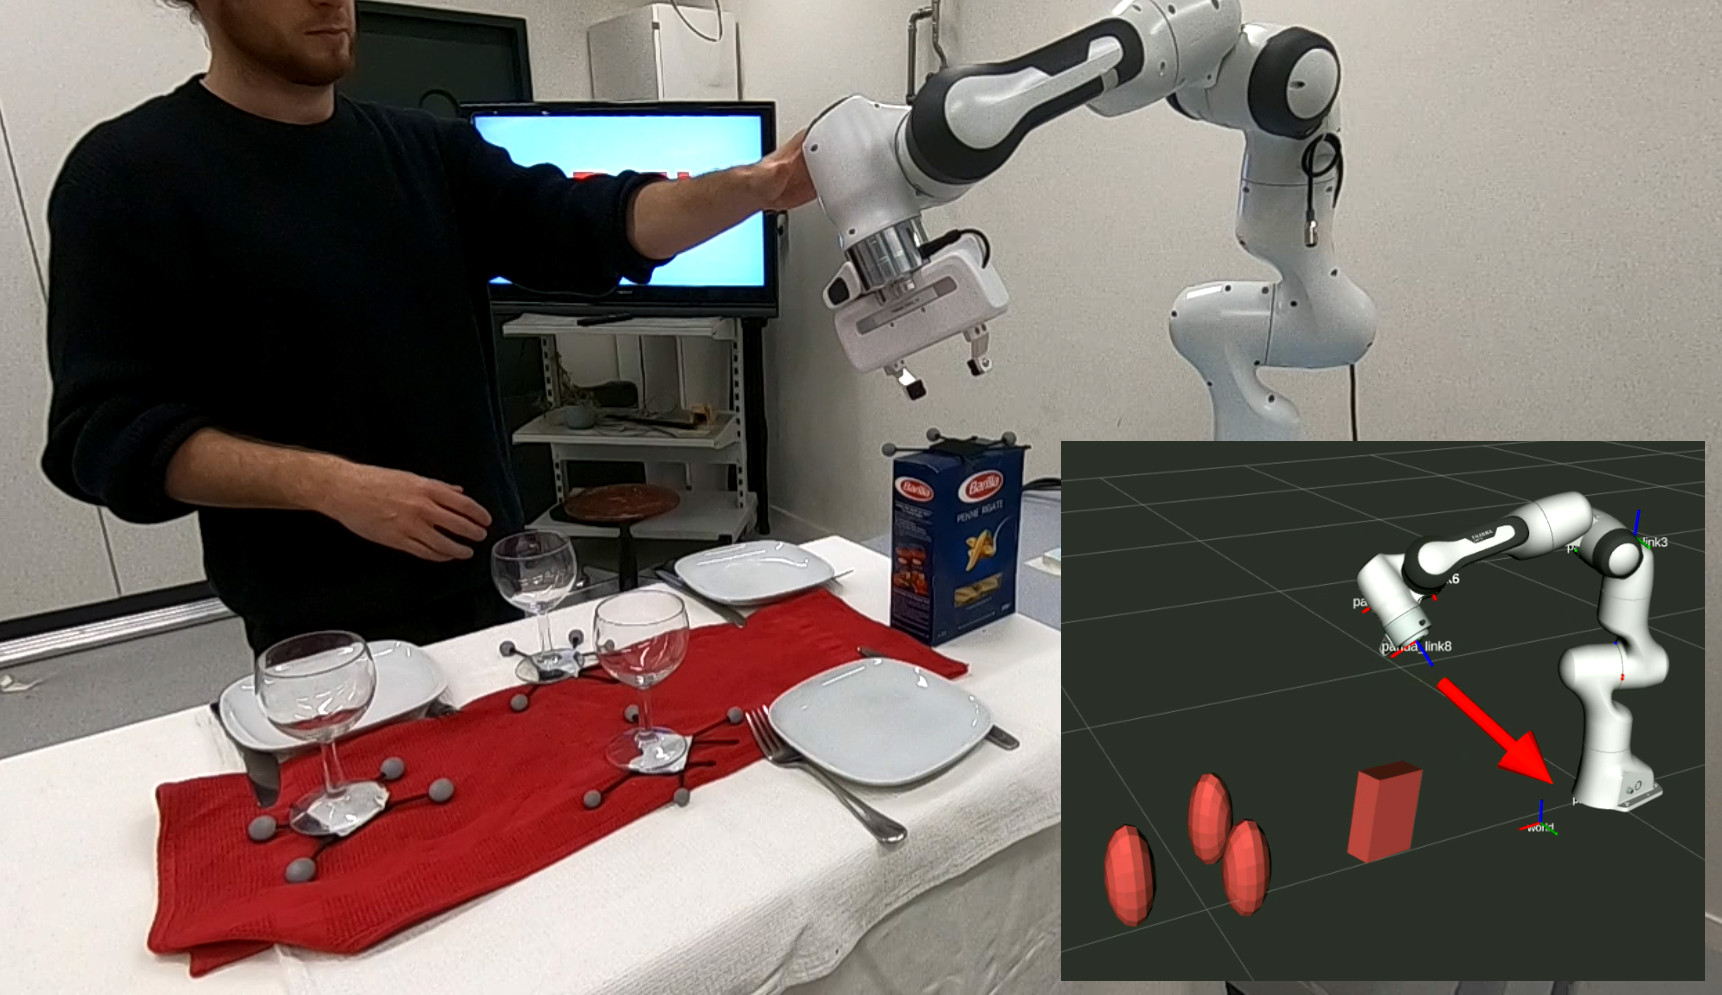
\includegraphics[width=0.5\textwidth]{figures/robot_arm_table_avoidance}}
\caption{
The proposed obstacle-aware passivity controller empowers the robot to evade external disturbances and maintain collision avoidance gracefully. 
Tipping over the closed pasta box on this dinner table setup might be acceptable, but handling delicate wine glasses demands care to prevent breakage.
}
\label{fig:table_avoidance_with_obstacle}
\end{figure}

In this paper, we present a novel approach to address these challenges and enhance the adaptability, reactivity, and safety of robotic movements. Our proposed method combines elements of DS control and impedance control, allowing the robot to navigate complex environments while proactively avoiding collisions and adeptly rejecting disturbances. We evaluate the performance of our approach through extensive simulations and practical implementation on a 7DoF robot arm, demonstrating its superiority over traditional methods in achieving robust and safe robot control in real-world scenarios.


\subsection{Related Work}
Impedance control, a powerful feedback algorithm, effectively applies Cartesian impedance to nonlinear manipulators' end-points \cite{takegaki1981new, hogan1985impedance}. By doing so, it replaces the computationally intensive \textit{inverse kinematics problem} with the more straightforward \textit{forward kinematics} approach. Unlike traditional position control algorithms, impedance control establishes a dynamic relationship between desired position, velocity, and force, offering a holistic control framework.
Initially, impedance controllers employed constant stiffness, but researchers have since explored various dynamic control parameter approaches to enhance adaptability in complex environments \cite{vanderborght2013variable, abu2020variable}.
% older variable actuators focused review \cite{vanderborght2013variable}
% Progress and prospects of the human-robot collaboration \cite{ajoudani2018progress}

% Passivity with increased precision
Passive velocity field controllers have emerged as a compelling technique for encoding desired tasks into velocity fields, combined with damping control laws to regulate robot movements. Stability can be guaranteed by using storage tanks inspired by a virtual flywheel \cite{li1999passive}. 
Learning and continuously adapting the control parameters have been shown to improve the controller performance in direct human-robot collaboration. 
\cite{gribovskaya2011motion}.
Increased convergence in passive controllers has achieved higher stiffness along the direction of motion but remains compliant otherwise \cite{kronander2015passive}. 
Alternative methods are combining impedance controllers with admittance controllers for increased accuracy in cooperative control
\cite{fujiki2022series}.
However, these controllers' adaptation focus on improving movement accuracy rather than actively rejecting disturbances.

% Stale interaction controller
Passive controller with stability based guaranteed using s storage tank function based on the system's energy allowed to limit contact force when interacting with the environment \cite{kishi2003passive}.
A general framework can be used to ensure that position-, torque-, and impedance controllers exhibit passive \cite{albu2007unified}. By interpreting the torque feedback as the shaping of the motor inertia, the flexible robot arms can be used in complex interaction tasks, such as insertion or wiping.
% Telemanipulation
Teleoperated systems of robot arms come with control delays and require a closed-loop controller of n robot that can adapt autonomously, ensuring stable and reliable performance. Passive controllers present themselves perfectly for such a task  \cite{stramigioli2005sampled}. This method addresses the intricate dynamics of interactive systems, ensuring stable and reliable performance.
A similar approach involves slowly updating the desired position while incorporating a spring-damper model through an impedance controller, enabling seamless interaction with the system \cite{lee2010passive}.
However, these models require a human in the loop for collision avoidance.

% Energy tanks 
Most presented impedance controllers with time-varying control rely on energy tanks to ensure stability. 
It follows from the fact, that varying parameters can increase the energy of the system \cite{ferraguti2013tank}. However, the energy tank when full can interfere with a controller's optimal functioning, and hence it cannot achieve a desired goal, such as collision avoidance.
Alternative approaches limit the impedance controller variables  by setting constraints on the damping and stiffness, as well as their rate of change based on a Lyapunov function \cite{kronander2016stability}.
% The controller was extended to have variable stiffness to favor task completion \cite{kronander2015passive}. However, both approaches rely on energy tanks for general, desired dynamics and do not give any guarantees in the presence of obstacles.

% Geometric Methods for Obstacle Avoidance / Force Control
Traditional tracking controllers often require complex linearization or simplification methods. However, a class of geometric tracking controllers enables exact control of nonlinear mechanical systems with low computational cost \cite{udwadia2003new}. By reformulating control problems as a specific class of optimal controllers, this approach facilitates the derivation of standard control problems in robotics \cite{peters2008unifying}.
Integrating local Riemannian Motion Policies (RMP) has led to globally stable force-controlled motion \cite{cheng2020rmp}. Moreover, recent advancements in position-dependent Riemannian metrics have improved task design using RMP, allowing for reactive force control under constraints \cite{bylard2021composable}.
Geometric fabrics have emerged as a valuable mathematical tool for shaping a robot's nominal behavior while capturing essential constraints like obstacle avoidance, joint limits, and redundancy resolution \cite{xie2020geometric}. The combination of Finsler geometry and geometric fabrics has further enhanced path consistency \cite{ratliff2021generalized}.
Integrating geometric fabric methods into classical mechanical systems has unlocked novel physical behaviors, notably exemplified in multi-obstacle avoidance for a 7DoF robot arm \cite{van2022geometric}. Despite these significant achievements, the parameterization of geometric methods remains challenging and can potentially introduce undesired motion artifacts.

% Tracking controllers often require linearization or other simplification methods. However, \cite{udwadia2003new} develops a class of tracking controllers for exact control of the nonlinear mechanical systems at a low computational cost by reformulating control problems as a particular class of optimal controllers. With this method, several standard control problems in robotics can be derived \cite{peters2008unifying}.
% The consistent combination of local Riemannian Motion Policies (RMP) is combined for globally stable force-controlled motion \cite{cheng2020rmp}.
% New position-dependent Riemannian metrics improve the task design using RMP, allowing for reactive force control under constraints \cite{bylard2021composable}.
% Geometric fabrics have been introduced as a mathematical tool for shaping the robot's nominal behavior, capturing constraints such as obstacle avoidance, joint limits, redundancy resolution
% \cite{xie2020geometric}.
% Finsler geometry combined with geometric fabrics has enabled increased path consistency \cite{ratliff2021generalized}.
% Geometric fabric generalizes classical mechanical systems to form new physical behavior, which has been used for multi-obstacle avoidance on a 7DoF robot arm \cite{van2022geometric}.
% However, the geometric methods remain challenging to parameterize and can create unwanted motion artifacts.
 % Real-time perception meets reactive motion generation \cite{kappler2018real} -> no real feedback on the collision avoidance level ?!

% AFP / Obstacle avoidance / Motion Control
In dynamic environments, obstacle avoidance is critical in ensuring safe robot navigation. Early approaches utilized repulsive force fields from robots to avoid collisions of robotic manipulators \cite{khatib1987unified}. 
% However, this method's susceptibility to local minima prompted the introduction of the elastic band method. By interpreting the initial trajectory as an elastic band and stretching the path around obstacles, this technique significantly improved convergence \cite{brock2002elastic}.
However, this method's susceptibility to local minima prompted the introduction of navigation functions: local minima are avoided a global (potential) function which the robot decends to reach the goal \cite{koditschek1990robot}. However, such functions depend on the distribution of the obstacles and are hard to adapt to dynamic environments and high dimensional spaces \cite{loizou2022mobile}.
% By interpreting the initial trajectory as an elastic band and stretching the path around obstacles, this technique significantly improved convergence \cite{brock2002elastic}.

% \cite{brock2002task}, % Corresponding conference 
Passive controllers have also been designed to track the curve of the general potential field while compensating for Coriolis and centrifugal forces. Nonetheless, these methods lack the guarantee of disturbance repulsion around obstacles \cite{duindam2004passive}. To address this, the integration of circular fields \cite{singh1996real} has allowed force-controlled navigation in cluttered environments, yielding increased convergence for simple obstacles \cite{haddadin2010real, haddadin2011dynamic}. This approach has been further combined with force-controlled navigation for manipulators \cite{tulbure2020closing}. 
However, it is important to note that this method's limitation to convex meshes and does not ensure the absence of local minima in space.

% In dynamic environments, obstacle avoidance is crucial for safe navigation. Early approaches used repulsive force fields from robots to avoid collisions of robotic manipulators \cite{khatib1987unified}. 
% As this approach is prone to local minima, the elastic band's method has been introduced. Interpreting the initial trajectory as an elastic band and stretching the path around obstacles improves convergence  
% \cite{
% % brock2002task, % Corresponding conference paper
% brock2002elastic}.
% Passive controllers have been designed to track the curve of the general potential field. The controller compensates for Coriolis and centrifugal forces. However, the method does not provide insurance of disturbance repulsion around obstacles \cite{duindam2004passive}. 
% The additional usage of circular fields \cite{singh1996real} allows force-controlled navigation in cluttered environments with increased convergence for simple obstacles
% \cite{haddadin2011dynamic}.
% This has been combined with force-controlled navigation for manipulators \cite{tulbure2020closing}. However, the method was limited to convex meshes and cannot guarantee the absence of local minima in space.

% Dynamical system based avoidance + control
In our prior work \cite{huber2019avoidance, huber2023avoidance}, we introduced a collision avoidance approach inspired by a harmonic potential. By design, this method guarantees the absence of local minima in free space, enabling effective navigation around complex scenarios, even in the presence of star-shaped obstacles.
While implementing a real robot, we utilized a passive controller that closely adheres to the desired velocity \cite{kronander2015passive}. However, one of the limitations of the passive controller is its inability to account for the physical surroundings fully. This makes the robot susceptible to disturbances in close proximity to obstacles, potentially leading to collisions.

% Alternatively, in our previous work \cite{huber2019avoidance, huber2023avoidance}, we introduced collision avoidance inspired by a harmonic potential. We ensured the absence of local minima in free space and enabled navigation around complex scenarios with star-shaped obstacles.
% For implementation on the real robot, a passive controller stays close to the initial dynamics \cite{kronander2015passive}. However, the passive controller does not take into account its physical surrounding, and disturbances in the proximity of obstacles could lead to collisions.

Although DS passive-controlled robots work well in interactive scenarios, they cannot ensure to navigate through an obstacle environment safely. For example, they often give in when being pushed toward an obstacle. This work presents a method to address this problem by modifying the passive control law design, resulting controller is now aware of its environment.

\subsection{Contribution}
In this work, we introduce a passive controller as visualized in Figure~\ref{fig:control_scheme_passive}. We make the following contributions:

\begin{itemize}
\item The design of a passive controller which ensures obstacle avoidance (Section~\ref{sec:obstacle_aware_passivity})
\item A passivity guarantee without the need for a storage tank which applies to general damping controller vector fields (Theorem~\ref{theorem:passivity})
\item A collision avoidance analysis which provides insight into the path consistency around obstacles (Section~\ref{sec:collision_avoidance})
\item Discrete-time analysis to ensure stability based on control parameters (Section~\ref{sec:discrete_time_behavior})
\item Implementation and testing on 7DoF robot arm (Section~\ref{sec:evaluation})
\end{itemize}

\begin{figure}[thb]
  \center
  \includesvg[width=1.0\columnwidth]{figures/control_scheme_passive.svg}
\caption{The desired velocity $\vect f^b(\vecs \xi)$ can result from a learned velocity field or pointing towards a desired attractor $\vecs \xi^a$. It is used to evaluate the obstacle avoidance velocity $\vect f(\vecs \xi)$, which is fed into the force controller to obtain the control force $\vect \tau_c$.}
\label{fig:control_scheme_passive}
\end{figure}
